\chapter{AC-MOT: Adaptive Detector Operating-Point Control}\label{ch:acmot}

\section{Introduction}\label{sec:ac-intro}
Multi-object tracking in UAV video is difficult because object density, size, illumination, and blur change over time, while most tracking-by-detection systems run the detector with fixed settings (Chapter~\ref{ch:intro}). This chapter presents the first controller of the thesis, Adaptive Control for Multi-Object Tracking (AC-MOT), a training-free controller that adjusts the detector operating point online: the confidence threshold, the IoU threshold of NMS, and the input resolution. Using only the current frame and the past output of the tracker, it selects one of three operating points without modifying or retraining the detector or the tracker. The chapter is based on the manuscript submitted to the Journal of Aerospace Information Systems \cite{ismail2026acmot}.

The evaluation shows that this simple control has a large effect. On the VisDrone2019 dataset with ByteTrack, the controller raised, relative to a fixed operating point, the HOTA by 7.1\%, the MOTA by 182\%, and the IDF1 by 11.0\%, and it reduced identity switches by 24.2\%. With OATrack, the same three scores rose by 2.8\%, 22.4\%, and 4.0\%, and identity switches fell by 21.9\%. Paired bootstrap analysis supports these improvements. On a second aerial benchmark, UAVDT, the controller raised MOTA with both trackers without retuning, including a 16.7\% gain with OATrack, and it adds about 4.2 ms per frame on a Tesla T4 GPU.

Section~\ref{sec:ac-problem} formulates the control problem and the requirements of the controller. Section~\ref{sec:acmot} presents the controller: its scene cues, the scene complexity index, the three-state controller, the action map, and the selection of its values. Section~\ref{sec:ac-dev} explains how optimization experiments on calibration data led to the frozen controller. Section~\ref{sec:ac-setup} describes the experimental setup, Section~\ref{sec:ac-results} gives the results on VisDrone2019-MOT and UAVDT, Section~\ref{sec:ac-discussion} discusses them, and Section~\ref{sec:ac-summary} summarizes the chapter.

\section{Problem Formulation and Design Requirements}\label{sec:ac-problem}
The detector settings at frame $t$ are called the operating point
\begin{equation}
\theta_t = (c_t, \eta_t, r_t),
\label{eq:ac-theta}
\end{equation}
which has three parts (Section~\ref{sec:bg-detection}):
\begin{itemize}
\item $r_t$ is the input resolution, the long side of the resized image in pixels. A larger input shows small objects better but takes more time.
\item $\eta_t$ is the NMS IoU threshold. When two boxes overlap with an IoU above $\eta_t$, the box with the lower score is removed. A lower $\eta_t$ removes more overlapping boxes.
\item $c_t$ is the score threshold. Boxes with a detector score below $c_t$ are removed before they reach the tracker. A higher $c_t$ passes fewer but more reliable boxes.
\end{itemize}
The detector weights and the tracker are frozen; the controller changes only $\theta_t$. It uses only information that is available at run time:
\begin{equation}
\theta_t = \pi\left(I_t, \mathcal{B}_{1:t-1}\right),
\label{eq:ac-policy}
\end{equation}
where $\pi$ is the control rule, $I_t$ is the image of the current frame, and $\mathcal{B}_{1:t-1}$ are the boxes that the tracker reported for the earlier frames $1$ to $t-1$. The tracker output of frame $t$ is used only from frame $t+1$ on. No ground truth, no future frame, and no detector score enters the decision.

The rule $\pi$ belongs to a family of rules with a small number of values (Section~\ref{sec:ac-constants}), and the operating points it may select come from a finite set of supported values. Its quality is judged by tracking, not by detection: in the final development stage, each candidate rule was scored by the cross-validated mean change in HOTA over a fixed operating point on separate calibration sequences,
\begin{equation}
J(\pi)=\frac{1}{F}\sum_{f=1}^{F}\left(\mathrm{HOTA}_f(\pi)-\mathrm{HOTA}_f(\theta_0)\right),
\label{eq:ac-objective}
\end{equation}
where $f$ runs over the $F=4$ cross-validation folds, $\mathrm{HOTA}_f$ is measured on the sequences held out in fold $f$, and $\theta_0$ is the fixed baseline operating point. The frozen rule was then chosen among the candidates that really adapt within the video (Section~\ref{sec:ac-modern}).

The controller must meet five requirements, which follow from the challenges of Section~\ref{sec:intro-motivation}:
\begin{enumerate}
\item \emph{Training-free and label-free:} no learned model and no ground truth at run time.
\item \emph{Causal:} the decision for frame $t$ uses only frames up to $t$ and tracker output up to $t-1$ (Eq.~\eqref{eq:ac-policy}).
\item \emph{External:} the detector and the tracker are used as they are; only three arguments of the detector call change.
\item \emph{Stable:} the operating point follows lasting changes of the scene, not single frames.
\item \emph{Inexpensive:} the cost of the controller is small next to the detector.
\end{enumerate}

\section{The AC-MOT Controller}\label{sec:acmot}
AC-MOT is a small, rule-based controller that runs next to the detector. On frame 1 and then on every tenth frame, it measures cheap cues of the current image and of the boxes tracked in the previous frame (Section~\ref{sec:ac-cues}), averages the recent crowd level into a scene complexity index (SCI) (Section~\ref{sec:ac-sci}), chooses a target state (LOW, MEDIUM, or HIGH), adjusts it with a recovery probe and hysteresis and dwell rules (Section~\ref{sec:ac-states}), and maps the state to one of three fixed detector operating points (Section~\ref{sec:ac-actions}). Section~\ref{sec:ac-constants} explains how each value is chosen. Figure~\ref{fig:ac-pipeline} shows where AC-MOT sits in the pipeline: the controller chooses the detector settings before the detector runs, and the detector and the tracker then run as usual.

\begin{figure}[tbp]
\centering
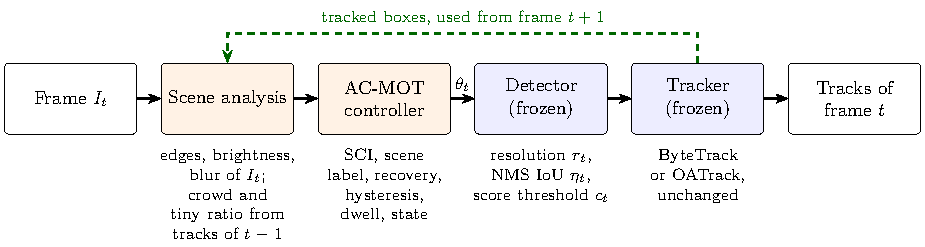
\includegraphics[width=0.98\textwidth]{figures/acmot_pipeline.pdf}
\caption{AC-MOT in a tracking-by-detection pipeline. Scene analysis and the controller choose the operating point $\theta_t=(c_t,\eta_t,r_t)$ before the detector runs. The frozen detector and tracker are not modified. Tracked boxes of frame $t$ feed the scene analysis of later frames (dashed arrow).}
\label{fig:ac-pipeline}
\end{figure}

\subsection{Scene Cues}\label{sec:ac-cues}
The controller needs a cheap description of the scene. Scene analysis therefore does not run on every frame. It runs on frame 1 and then once every 10 frames ($t=1$ or $t \bmod 10 = 1$, that is, frames 1, 11, 21, \dots). Each of these frames is an analysis step $j$. Between two analysis steps the controller keeps its last decision. Two kinds of cues are computed at each step: image cues, which describe how the current frame looks, and box cues, which describe the objects that the tracker found in the previous frame.

\emph{Image cues of the current frame.} The frame is reduced to a quarter of its width and height and converted to gray levels, so that the cues are cheap to compute. Three cues are then measured:
\begin{itemize}
\item the edge density $e_t$, the fraction of pixels marked as edges by the Canny detector (lower and upper thresholds 50 and 120); many edges indicate a cluttered scene;
\item the brightness $\beta_t$, the mean gray level from 0 (black) to 255 (white); a low value indicates a dark or night scene;
\item the sharpness $\nu_t$, the variance of the Laplacian of the gray image \cite{pechpacheco2000blur}; a low value indicates a blurred frame.
\end{itemize}

\emph{Box cues of the previous frame.} Let $N_j$ be the number of boxes that the tracker reported for frame $t-1$, and let $a_i$ be the area of box $i$ in pixels of the original image. The crowd cue and the tiny-object ratio are
\begin{align}
C_j&=\min\!\left(\frac{N_j}{30},1\right),\label{eq:ac-crowd}\\
T_j&=\frac{1}{N_j}\sum_{i=1}^{N_j}\mathbf{1}\!\left[a_i<32^2\right].\label{eq:ac-tiny}
\end{align}
$C_j$ is the number of tracked objects divided by 30 and capped at 1, so every frame with 30 or more objects has $C_j=1$. $T_j$ is the fraction of tracked boxes smaller than $32\times32$ pixels, which is the size limit of small objects in the COCO benchmark \cite{lin2014coco}. The indicator $\mathbf{1}[\cdot]$ is 1 when its condition holds and 0 otherwise, and $T_j=0$ when $N_j=0$.

\subsection{Scene Complexity Index and Scene Label}\label{sec:ac-sci}
The SCI measures how crowded the recent frames are. A single frame is a noisy measurement, because the tracker may miss or add a few objects in any frame, so the SCI averages over time. It is the mean crowd cue of the last seven analysis steps:
\begin{equation}
S_j=\frac{1}{|H_j|}\sum_{k\in H_j} C_k,
\label{eq:ac-sci}
\end{equation}
where $H_j$ holds the steps $j-6,\dots,j$ (fewer at the start of a video) and $|H_j|$ is their number. With a stride of 10 frames, the seven steps cover about the last 60 frames, so a single unusual frame changes $S_j$ only a little. Because $C_j\le1$, $S_j$ lies between 0 and 1.

The SCI uses the crowd cue alone, selected by the cue audit of Section~\ref{sec:ac-modern}. The other four cues are still used as checks on the state, mainly through the scene label
\begin{equation}
\ell_j=\begin{cases}
\text{night}   & \text{if } \beta_t<80,\\
\text{blur}    & \text{else if } \nu_t<180,\\
\text{tiny}    & \text{else if } T_j>0.50,\\
\text{crowded} & \text{else if } C_j>0.65 \text{ or } e_t>0.13,\\
\text{clear}   & \text{otherwise.}
\end{cases}
\label{eq:ac-label}
\end{equation}
The conditions are checked from top to bottom, and the first one that holds gives the label. For example, $T_j>0.50$ means that more than half of the tracked boxes are tiny, and $C_j>0.65$ means that at least 20 objects are tracked.

Only the crowd cue enters the SCI, and it also enters the crowded label. The tiny-object ratio $T_j$ is used by the state rules of Section~\ref{sec:ac-states} and gives the tiny label, and the edge density $e_t$ is used only through the crowded label. The brightness $\beta_t$ and the sharpness $\nu_t$ act only through the night and blur labels, which do not lead to MEDIUM or HIGH by themselves: because they are checked first, a dark or blurred frame cannot receive the crowded or tiny label, while the SCI conditions and the tiny-object guard of Eq.~\eqref{eq:ac-target} still apply.

\subsection{Three-State Controller}\label{sec:ac-states}
The controller is always in one of three states: LOW, MEDIUM, or HIGH. The names describe the scene: LOW for a sparse scene, HIGH for a crowded scene or a scene of mostly tiny objects. They do not rank the input size: in the final action map the HIGH state uses the smallest input (Table~\ref{tab:ac-actions}). The state is updated only at analysis steps, in four steps (Algorithm~\ref{alg:ac-controller}). Step~1 proposes a target state from the cues. Steps~2--4 adjust this target so that the controller reacts to a sudden drop in the object count but does not switch back and forth.

\emph{Step 1: target state.} The target is the state that the current cues ask for. It is given by the SCI, the tiny-object ratio, and the scene label:
\begin{equation}
g_j=\begin{cases}
\text{HIGH}   & \text{if } S_j>\tau_h \text{ or } T_j>0.50,\\
\text{MEDIUM} & \text{else if } S_j>\tau_m \text{ or } \ell_j\in\{\text{crowded},\text{tiny}\},\\
\text{LOW}    & \text{otherwise,}
\end{cases}
\label{eq:ac-target}
\end{equation}
where $\tau_m=0.297$ and $\tau_h=0.511$ are the two SCI thresholds (Table~\ref{tab:ac-constants}). Since $S_j$ is the recent average number of tracked objects divided by 30, the SCI conditions give MEDIUM above about 9 objects ($30\tau_m=8.9$) and HIGH above about 15 objects ($30\tau_h=15.3$).

\emph{Step 2: recovery probe.} The SCI averages seven steps, so it reacts slowly when the tracker suddenly reports far fewer objects than a few steps earlier. The recovery probe responds to such a collapse of the object count. Instead of letting the falling count move the controller toward a lower state, it sets the target to HIGH for a short time. To detect a collapse, it keeps a slowly decaying peak $P_j$ of the object count and a drop counter $d_j$:
\begin{align}
d_j&=\begin{cases}
d_{j-1}+1 & \text{if } P_{j-1}\ge5 \text{ and } N_j<0.40\,P_{j-1},\\
0         & \text{otherwise,}
\end{cases}\label{eq:ac-drop}\\
P_j&=\max\left(N_j,\lfloor 0.8\,P_{j-1}\rfloor\right),\label{eq:ac-peak}
\end{align}
with $P_0=d_0=0$. A collapse is detected when at least 5 objects have been seen before and fewer than 40\% of them remain. The peak loses 20\% at each step, so an old peak is forgotten after a few steps. While $1\le d_j\le3$, the target $g_j$ is set to HIGH, so the probe lasts at most three analysis steps (30 frames); the dwell rule of Step~4 still applies.

\emph{Step 3: hysteresis.} Without a margin, a scene whose SCI stays close to a threshold would make the controller switch at almost every step. Hysteresis prevents this: a move to a lower state is held while the scene is still close to difficult:
\begin{equation}
g_j\leftarrow\begin{cases}
\text{HIGH}   & \text{if } q_{j-1}=\text{HIGH} \text{ and } (S_j>0.50 \text{ or } T_j>0.40),\\
\text{MEDIUM} & \text{if } q_{j-1}=\text{MEDIUM},\ g_j=\text{LOW} \text{ and } S_j>0.25,\\
g_j           & \text{otherwise.}
\end{cases}
\label{eq:ac-hold}
\end{equation}
The hold values lie just below the values that lead into each state ($0.50<\tau_h$, 0.40 below the tiny guard of 0.50, and $0.25<\tau_m$). Upward moves are not held.

\emph{Step 4: dwell.} The dwell rule sets a minimum time between two changes. After a change, the state is kept for at least 30 frames, that is, three analysis steps:
\begin{equation}
q_j=\begin{cases}
g_j     & \text{if } t-t_c\ge30,\\
q_{j-1} & \text{otherwise,}
\end{cases}
\label{eq:ac-dwell}
\end{equation}
where $t_c$ is the frame of the last state change. The controller starts in LOW with $t_c=1$, so the first change is possible at frame 31. Whenever $q_j\ne q_{j-1}$, $t_c$ is set to $t$.

\emph{Why changes are kept rare.} Each change of state changes the boxes that reach the tracker, so the temporal rules let the state follow lasting changes of the scene, not single frames: the seven-step window smooths the SCI over about 60 frames, the holds add a margin below each threshold, and the dwell rule allows at most one change every 30 frames.

\emph{Example.} Consider a clear, sharp video in which the tracker reports 20 objects of normal size in every frame ($C_j=0.67$), and only 10 objects from frame 71 on. The controller starts in LOW. The first step sees no earlier boxes ($C_j=0$), so $S_j$ grows as the window fills: 0.33 at frame 11, 0.44 at frame 21, and 0.50 at frame 31. The target is MEDIUM from frame 11, but the dwell rule keeps LOW until frame 31, where the state becomes MEDIUM. From frame 41, $S_j$ exceeds $\tau_h$ and the target is HIGH; the dwell rule delays this change to frame 61. When the scene thins, $S_j$ falls slowly because the window still holds the earlier steps, so the state stays HIGH until frame 101. At frame 111, $S_j=0.48$ is below both $\tau_h$ and the hold value of 0.50, and the state returns to MEDIUM. It then stays in MEDIUM, because 10 tracked objects keep $S_j$ at about 0.33, above $\tau_m$.

The state $q_j$ then selects the operating point from the action map, and the detector uses it until the next analysis step.

\begin{algorithm}[tbp]
\caption{AC-MOT controller for one video.}\label{alg:ac-controller}
\begin{algorithmic}[1]
\Require frames $I_1, I_2, \dots$; frozen detector and tracker; constants of Table~\ref{tab:ac-constants}
\Ensure tracks of every frame
\State $j\gets0$; $q_0\gets$ LOW; $P_0\gets0$; $d_0\gets0$; $t_c\gets1$
\For{each frame $t=1,2,\dots$}
  \If{$t=1$ \textbf{or} $t \bmod 10=1$} \Comment{analysis step, every 10 frames}
    \State $j\gets j+1$
    \State $e_t,\beta_t,\nu_t\gets$ image cues of $I_t$ \Comment{Section~\ref{sec:ac-cues}}
    \State $N_j,C_j,T_j\gets$ cues of the tracked boxes of frame $t-1$ \Comment{no boxes at $t=1$}
    \State $S_j\gets$ mean of $C_k$ over the last seven steps $k\in H_j$ \Comment{SCI, Eq.~\eqref{eq:ac-sci}}
    \State $\ell_j\gets$ label, Eq.~\eqref{eq:ac-label}; $g_j\gets$ target, Eq.~\eqref{eq:ac-target} \Comment{Step 1: target}
    \State update $d_j$ and $P_j$, Eqs.~\eqref{eq:ac-drop}--\eqref{eq:ac-peak}
    \If{$1\leq d_j\leq3$} $g_j\gets$ HIGH \Comment{Step 2: recovery probe}
    \EndIf
    \State apply hysteresis to $g_j$, Eq.~\eqref{eq:ac-hold} \Comment{Step 3: hysteresis}
    \If{$t-t_c\geq30$ \textbf{and} $g_j\neq q_{j-1}$} \Comment{Step 4: dwell}
      \State $q_j\gets g_j$; $t_c\gets t$
    \Else
      \State $q_j\gets q_{j-1}$
    \EndIf
  \EndIf
  \State $(r_t,\eta_t,c_t)\gets$ action of state $q_j$, Table~\ref{tab:ac-actions} \Comment{kept until the next analysis step}
  \State detect with $r_t$ and $\eta_t$; drop boxes with score $<c_t$
  \State update the tracker; store its boxes of frame $t$ \Comment{used from frame $t+1$}
\EndFor
\end{algorithmic}
\end{algorithm}

\subsection{Action Map}\label{sec:ac-actions}
Table~\ref{tab:ac-actions} gives the operating point of each state. The actions are not set by hand: they are selected together with $\tau_m$ and $\tau_h$ by the joint search on the calibration sequences, whose objective is the change in HOTA, a metric that balances detection and association (Section~\ref{sec:ac-constants}).

In LOW, the sparse state, the detector uses the largest input, loose NMS, and a low score threshold, so it passes more weak boxes. In MEDIUM and HIGH it passes only boxes with a score of at least 0.40. The HIGH state, used for crowded scenes and for scenes of mostly tiny objects, thus has the smallest input. This may look surprising, since a larger input shows small objects better, but the search optimizes tracking quality, not the detection of every small object: a score threshold of 0.40 gives the tracker fewer but more reliable boxes (Section~\ref{sec:ac-modern}), and the smaller input costs less detector time. Section~\ref{sec:ac-results} shows that the main effect of AC-MOT is a more selective detection stream: fewer false positives and identity switches, with similar or slightly lower recall. This action is the result of the search, not a general rule that crowded scenes need smaller inputs.

The score threshold $c_t$ is applied on the detector side before the tracker. It is separate from any confidence gate inside the tracker, such as the fixed tracker-side gate of OATrack.

\begin{table}[tbp]
\centering
\caption{Action map of AC-MOT. State names describe scene difficulty, not a resolution rank. Selected by the joint search on the calibration sequences.}
\label{tab:ac-actions}
\begin{tabular}{lrrr}
\toprule
State & Resolution $r$ (pixels) & NMS IoU $\eta$ & Score threshold $c$\\
\midrule
LOW & 1536 & 0.70 & 0.10\\
MEDIUM & 1280 & 0.45 & 0.40\\
HIGH & 1088 & 0.60 & 0.40\\
\bottomrule
\end{tabular}
\end{table}

\subsection{Selection of Parameter Values}\label{sec:ac-constants}
All values of Tables~\ref{tab:ac-actions} and~\ref{tab:ac-constants} are fixed before the final evaluation and are not changed after it. The last column of Table~\ref{tab:ac-constants} gives the source of each value. There are four sources.

\emph{Joint search on the calibration sequences.} The SCI thresholds $\tau_m$ and $\tau_h$ and the action map are selected together by an Optuna TPE search with 60 trials \cite{akiba2019optuna}; the search ranges are given in Section~\ref{sec:ac-modern}. The calibration sequences are eight sequences of the VisDrone2019-MOT training split. They serve as the validation (tuning) data of the final stage and are disjoint from the evaluation sequences. Each trial is scored by four-fold cross-validation (CV), with two sequences held out in each fold, as the mean change in HOTA against the baseline. The candidate values come from existing settings. The input sizes (1088, 1280, and 1536 pixels) and NMS values (0.45, 0.60, and 0.70) are the operating points for which detector outputs are cached; 1536 pixels with NMS 0.70 is the baseline point, and 0.70 is the default NMS value of the Ultralytics detector. The three score thresholds are the low and high thresholds of ByteTrack (0.10 and 0.25) and the confidence gate of OATrack (0.40).

\emph{Cue audit on the calibration sequences.} The choice of the crowd cue as the only SCI input comes from testing all 31 non-empty subsets of the five cues with the same cross-validation (Section~\ref{sec:ac-modern}).

\emph{Temporal sweep on the validation split.} The analysis stride and the SCI window are selected in the first development stage, with the YOLOv8n pipeline, on the VisDrone2019-MOT validation sequences. The sweep tests 25 combinations: windows of 1, 3, 5, 7, and 9 analysis steps and strides of 1, 5, 10, 15, and 20 frames. Five of the 25 settings meet both constraints of that stage, at least 25 frames per second (FPS) and at most 271 identity switches (the number of the original controller on the same data). Among them, a window of 7 and a stride of 10 give the highest MOTA, 18.165 against 18.044 for the next setting. Operating-point sweeps on the same data cover input resolutions from 512 to 960 pixels, confidence thresholds from 0.05 to 0.50, and NMS thresholds from 0.30 to 0.80, and define the supported values of the first optimized profiles (Section~\ref{sec:ac-dev}).

\emph{Fixed design values.} The tiny-object area follows the COCO definition of small objects \cite{lin2014coco}. The remaining values (the crowd normalizer, the Canny thresholds, the label thresholds, the recovery, hold, and dwell values, and the initial state) come from the original AC-MOT controller and are kept unchanged in every search of the final stage, so the searched values are matched to them. For example, the crowd normalizer of 30 only sets the scale of $S_j$: $\tau_m$ and $\tau_h$ are searched on this scale and correspond to about 9 and 15 tracked objects.

\begin{table}[tbp]
\centering
\caption{Values of the AC-MOT controller and how each value is chosen. Calibration sequences: eight VisDrone2019-MOT training sequences used as tuning data, disjoint from the evaluation sequences. CV: four-fold cross-validation.}
\label{tab:ac-constants}
\begin{tabular}{>{\raggedright\arraybackslash}p{1.5cm}>{\raggedright\arraybackslash}p{4.3cm}>{\raggedright\arraybackslash}p{2.4cm}>{\raggedright\arraybackslash}p{5.2cm}}
\toprule
Symbol & Meaning & Value & How the value is chosen\\
\midrule
$\tau_m$ & SCI threshold for MEDIUM, Eq.~\eqref{eq:ac-target} & 0.297 & joint TPE search on the calibration sequences, 60 trials, CV\\
$\tau_h$ & SCI threshold for HIGH, Eq.~\eqref{eq:ac-target} & 0.511 & same joint search\\
$(r,\eta,c)$ & operating point of each state & Table~\ref{tab:ac-actions} & same joint search over $\{1088,1280,1536\}\times\{0.45,0.60,0.70\}\times\{0.10,0.25,0.40\}$\\
-- & SCI input cue & crowd only & cue audit of all 31 cue subsets on the calibration sequences, CV\\
-- & analysis stride & 10 frames & temporal sweep of 25 settings on the validation split; highest MOTA with $\geq$25 FPS and $\leq$271 IDS\\
$|H_j|$ & SCI window & 7 steps & same temporal sweep\\
-- & tiny-object area & $32\times32$ pixels & COCO small-object limit \cite{lin2014coco}\\
-- & crowd normalizer, Eq.~\eqref{eq:ac-crowd} & 30 boxes & original controller; sets the scale on which $\tau_m$, $\tau_h$ are searched\\
-- & Canny thresholds (lower, upper) & 50, 120 & original controller; fixed in all final-stage searches\\
-- & night and blur labels, Eq.~\eqref{eq:ac-label} & $\beta_t<80$, $\nu_t<180$ & original controller; fixed in all final-stage searches\\
-- & crowded label, Eq.~\eqref{eq:ac-label} & $C_j>0.65$ or $e_t>0.13$ & original controller; fixed in all final-stage searches\\
-- & tiny label and HIGH guard, Eqs.~\eqref{eq:ac-label}, \eqref{eq:ac-target} & $T_j>0.50$ & original controller; fixed in all final-stage searches\\
-- & recovery: minimum peak, drop ratio, peak decay, steps & 5, 0.40, 0.80, 3 & original controller; fixed in all final-stage searches\\
-- & holds in HIGH ($S_j$, $T_j$) and MEDIUM ($S_j$), Eq.~\eqref{eq:ac-hold} & (0.50, 0.40), 0.25 & original controller; fixed in all final-stage searches\\
-- & dwell, Eq.~\eqref{eq:ac-dwell} & 30 frames & original controller; fixed in all final-stage searches\\
-- & initial state & LOW & original controller; fixed in all final-stage searches\\
\bottomrule
\end{tabular}
\end{table}

\section{Development of the Frozen Controller}\label{sec:ac-dev}
The controller of Section~\ref{sec:acmot} is the result of four development stages. The quality-oriented profile (Section~\ref{sec:ac-quality}) asked whether a scene index that steers the detector settings can beat a fixed default; the identity-aware profile (Section~\ref{sec:ac-identity}) made identity stability and speed explicit objectives; the transfer studies (Section~\ref{sec:ac-transfer}) tested other data and pipelines; and the modern stage (Section~\ref{sec:ac-modern}) built the frozen controller for a modern detector with separate calibration data. The first three stages are historical: they used a weighted five-cue index with interpolated confidence and NMS values and three resolution levels (the SparseTrack study used a single edge-driven NMS rule), other detectors, and other evaluation protocols. Their numbers are reported in their own tables, each against its own baseline, and are not pooled with the modern results. Only the frozen controller of the final stage is evaluated in Section~\ref{sec:ac-results}. Within the final stage, the cue audit and the score-threshold sweep play the role of an ablation: they test which scene cues and which parts of the operating point the controller needs.

\subsection{Quality-Oriented Profile}\label{sec:ac-quality}
\emph{Baseline.} The reference pipeline is the pretrained YOLOv8n detector \cite{jocher2023yolov8} followed by ByteTrack \cite{zhang2022bytetrack}, both at their default settings: confidence threshold 0.25, NMS IoU threshold 0.45, input size 640 pixels, and the default ByteTrack parameters listed in Section~\ref{sec:ac-setup}. It runs with one fixed operating point for the whole video.

\emph{Method.} The first optimization-derived profile kept the same detector, used a tuned ByteTrack profile, and searched only on the VisDrone2019-MOT validation split. Each of five cues was normalized with validation statistics, and the index was their weighted sum
\begin{equation}
S_j=\sum_{k\in\{c,t,e,n,b\}}w_k\,x_{k,j},
\label{eq:ac-histsci}
\end{equation}
where $k$ runs over the cues (c: crowd count, t: fraction of earlier boxes below $32\times32$ pixels, e: edge density, n: low brightness, b: low Laplacian variance), $x_{k,j}$ is the normalized value of cue $k$ at analysis step $j$, and $w_k$ is its weight, with $w_k\geq0$ and $\sum_k w_k=1$. The index was averaged over seven analyses taken every ten frames. Confidence and NMS were interpolated linearly between the values at $S=0$ and $S=1$, and two sorted thresholds selected one of three resolutions (512, 928, 960 pixels).

An Optuna TPE study \cite{akiba2019optuna} jointly searched the five weights, the confidence and NMS end points, and the two thresholds. The resolution levels, the supported confidence values $\{0.25,\dots,0.45\}$, the supported NMS values from 0.30 to 0.70, and the temporal settings were fixed beforehand by validation sweeps (Section~\ref{sec:ac-constants}). The selection rule kept trials with at least 25 FPS and at most 271 IDS (the IDS of the original controller on the same validation data) and then took the highest MOTA, with lower IDS, HOTA, IDF1, and FPS as tie-breaks. The frozen profile (archived as Trial~24) has $w_c=0.1294928$, $w_t=0.2217477$, $w_e=0.4337134$, $w_n=0.0535577$, $w_b=0.1614885$, confidence end points $(0.30,0.40)$, NMS end points $(0.35,0.35)$, and thresholds $(0.1353494, 0.2872868)$. On validation it reached MOTA 23.038, HOTA 36.110, IDF1 40.758, and IDS 270 at 37.169 FPS.

\emph{Comparison.} Table~\ref{tab:ac-quality} compares the profile with the baseline on the historical VisDrone test-dev split, with paired bootstrap intervals (5000 resamples, seed 42). A scene index that steers the detector settings improved tracking quality over the fixed default point, with HOTA, MOTA, and IDF1 intervals above zero. The IDS interval, $[-114, 219]$, includes zero; the next stage made identity stability an explicit objective. The final controller keeps two parts of this stage: the stride of 10 frames and the window of seven steps from its temporal sweep (Section~\ref{sec:ac-constants}), and the five kinds of scene cues, which were audited again in the modern stage.

\begin{table}[tbp]
\centering
\caption{Quality-oriented profile versus its baseline (YOLOv8n with ByteTrack at default settings) on VisDrone test-dev, historical protocol. Gain: paired bootstrap difference with 95\% interval; for IDS it is the reduction.}
\label{tab:ac-quality}
\begin{tabular}{lrrl}
\toprule
Metric & Baseline & Quality & Gain [95\% CI]\\
\midrule
HOTA & 28.430 & 33.835 & $+5.4051$ [$4.1273$, $6.9022$]\\
MOTA & 19.729 & 26.948 & $+7.2195$ [$5.4362$, $9.2934$]\\
IDF1 & 32.724 & 41.546 & $+8.8220$ [$6.9005$, $11.0537$]\\
IDS & 1235 & 1184 & $51$ [$-114$, $219$]\\
FPS & 36.528 & 38.985 & --\\
\bottomrule
\end{tabular}
\end{table}

\subsection{Identity-Aware Pareto Profile}\label{sec:ac-identity}
\emph{Baseline.} The baseline is the same YOLOv8n and ByteTrack pipeline at default settings (Section~\ref{sec:ac-quality}).

\emph{Method.} The second study kept the same cues, operating levels, temporal settings, and validation data, but changed the question. It maximized MOTA and minimized IDS subject only to $\mathrm{FPS}\geq25$, without the IDS gate. A seeded TPE sampler ran 49 completed trials. A trial dominated another when it had no lower MOTA and no higher IDS, with at least one strict improvement, and the feasible Pareto front was built from these relations. The balanced candidate maximized an equal-weight score of normalized MOTA and normalized IDS reduction, with HOTA, IDF1, FPS, and trial index as tie-breaks. The selected profile (archived as Trial~22) has weights $w_c=0.1646453$, $w_t=0.1746265$, $w_e=0.5076113$, $w_n=0.1206956$, $w_b=0.0324213$, confidence end points $(0.40,0.40)$, NMS end points $(0.60,0.35)$, and thresholds $(0.2927136, 0.6661672)$. On validation it reached MOTA 19.330, HOTA 31.651, IDF1 34.226, and IDS 168 at 51.406 FPS.

\emph{Comparison.} Table~\ref{tab:ac-identity} compares the profile with the baseline on test-dev. It removes 316 IDS and raises throughput from 36.528 to 46.024 FPS, while HOTA, MOTA, and IDF1 also rise. Against the quality-oriented profile it has 265 fewer IDS $[82, 502]$ and $-2.617$ HOTA $[-4.004, -1.694]$. The two profiles therefore answer different questions: one favors overall quality and the other favors identity stability and speed. The detector operating point controls a trade-off between quality, identity stability, and speed, and the objective of the search decides which side is favored.

\begin{table}[tbp]
\centering
\caption{Identity-aware profile versus its baseline (YOLOv8n with ByteTrack at default settings) on VisDrone test-dev, historical protocol. Gain: paired bootstrap difference with 95\% interval; for IDS it is the reduction.}
\label{tab:ac-identity}
\begin{tabular}{lrrl}
\toprule
Metric & Baseline & Identity & Gain [95\% CI]\\
\midrule
HOTA & 28.430 & 31.218 & $+2.788$ [$0.747$, $4.660$]\\
MOTA & 19.729 & 23.792 & $+4.063$ [$0.952$, $6.886$]\\
IDF1 & 32.724 & 37.870 & $+5.146$ [$2.028$, $8.080$]\\
IDS & 1235 & 919 & $316$ [$175$, $470$]\\
FPS & 36.528 & 46.024 & --\\
\bottomrule
\end{tabular}
\end{table}

\subsection{Transfer and Cross-Pipeline Studies}\label{sec:ac-transfer}
This stage applied the historical controllers outside their development setting: to a second dataset, and to two other detector--tracker pipelines.

\emph{UAVDT.} The baseline is again YOLOv8n with ByteTrack at default settings (Section~\ref{sec:ac-quality}). Both frozen profiles were applied to UAVDT \cite{du2018uavdt} without retuning (Table~\ref{tab:ac-histuavdt}). The quality-oriented profile raised HOTA by 4.305 points $[2.740, 5.709]$ and the identity-aware profile by 2.845 points $[1.238, 4.348]$; their IDS reductions are 237 $[104, 377]$ and 250 $[110, 404]$.

\begin{table}[tbp]
\centering
\caption{Historical UAVDT transfer without retuning. Baseline: YOLOv8n with ByteTrack at default settings.}
\label{tab:ac-histuavdt}
\begin{tabular}{lrrr}
\toprule
Metric & Baseline & Quality & Identity\\
\midrule
HOTA & 24.085 & 28.390 & 26.930\\
MOTA & 13.841 & 17.399 & 16.118\\
IDF1 & 27.887 & 34.453 & 32.014\\
IDS & 558 & 321 & 308\\
FPS & 65.015 & 58.353 & 61.462\\
\bottomrule
\end{tabular}
\end{table}

\emph{U2MOT on VisDrone.} The baseline is the published U2MOT tracker \cite{liu2023u2mot} with its released YOLOX-X detector, run at its own static setting. Seven VisDrone validation sequences served for development and 17 test-dev sequences for evaluation. The cue weights and transforms of the quality-oriented profile were kept, the tracker was not modified, and the action boundaries were set to the 33rd and 67th percentiles of the index on the U2MOT validation run, without using ground truth. Table~\ref{tab:ac-u2mot} (top) gives the comparison: the controlled pipeline has 87 fewer IDS and 1230 fewer false positives, while MOTA is almost unchanged and false negatives are higher.

\emph{SparseTrack on MOT17.} The baseline is the published SparseTrack tracker \cite{liu2025sparsetrack} with a fixed NMS IoU threshold of 0.75, on the seven MOT17 val-half sequences (2652 frames) \cite{dendorfer2021motchallenge}. A minimal edge-driven rule switched only the NMS threshold, between 0.70 and 0.80; its threshold came from a leave-one-sequence-out study on the same sequences. Table~\ref{tab:ac-u2mot} (bottom) gives the comparison: the adaptive rule reduces IDS from 136 to 123, with MOTA $+0.0371$ points $[-0.041, +0.182]$.

\begin{table}[tbp]
\centering
\caption{Cross-pipeline studies. Top: U2MOT with its YOLOX-X detector at its static setting on VisDrone test-dev. Bottom: SparseTrack with a fixed NMS IoU threshold of 0.75 on MOT17 val-half.}
\label{tab:ac-u2mot}
\begin{tabular}{llrr}
\toprule
Pipeline & Metric & Baseline & With control\\
\midrule
U2MOT & MOTA & 53.873 & 53.767\\
 & IDF1 & 69.775 & 69.849\\
 & IDS & 1239 & 1152\\
 & FP & 41385 & 40155\\
 & FN & 63241 & 64801\\
\midrule
SparseTrack & MOTA & 76.8881 & 76.9252\\
 & IDF1 & 81.4943 & 81.5299\\
 & IDS & 136 & 123\\
\bottomrule
\end{tabular}
\end{table}

The frozen profiles kept their direction on UAVDT without retuning, and with U2MOT and SparseTrack the control mainly reduced IDS, with small changes in MOTA. Together these studies show that the preferred profile depends on the objective (quality or identity) and on the tracker host. This motivated a modern stage with a stronger detector, explicit calibration data, and two tracker hosts.

\subsection{Modern Stage}\label{sec:ac-modern}
The modern stage decided which cues enter the SCI, which operating points each state uses, and where the SCI thresholds lie.

\emph{Baseline.} The modern baseline is the YOLO11m detector \cite{jocher2024yolo11}, in a public version trained on VisDrone2019-DET \cite{zhu2022visdrone}, run at a fixed operating point of 1536 pixels and NMS IoU 0.70 with no extra score threshold. It feeds ByteTrack \cite{zhang2022bytetrack} during development and both ByteTrack and OATrack \cite{qi2026oatrack} in the final evaluation. A large fixed input is a common choice for small aerial objects when no adaptation is used.

\emph{Data and protocol.} Eight sequences of the VisDrone2019-MOT training split (3282 frames) were declared as calibration data. They are disjoint from the seven evaluation sequences. The searches used the same four folds, each holding out two calibration sequences. Detector outputs were cached for every resolution and NMS value; a score threshold applied to the cache was checked to reproduce direct inference exactly. The steps are described below in the order in which they were carried out.

\emph{Resolution and NMS maps.} Two exhaustive grid searches, archived as Stages 1 and 2, searched the state-to-resolution and state-to-NMS maps. At this point the action of a state contained only the input resolution and the NMS value.

\emph{Cue audit.} The next search, archived as Stage 3A, asked which cues should form the SCI. It searched all 31 non-empty subsets of the five cues and selected \{crowd\}, which defines the crowd-selected SCI of Eq.~\eqref{eq:ac-sci}. The other cues were kept as guard and auxiliary cues of the state logic (Section~\ref{sec:ac-sci}).

\emph{Score threshold.} A separate sweep then tested the score threshold. At 1088 pixels and NMS 0.45, a fixed score threshold of 0.40 raised pooled calibration HOTA by $+0.881$ over 0.01 and improved seven of the eight sequences. The score threshold was therefore added as the third action dimension.

\emph{Final joint search.} The final search then selected the thresholds and the three-part actions together. It used 60 TPE trials (seed 43) and searched $\tau_m\in[0.10,0.50]$, $\tau_h\in[\tau_m+0.05,\min(\tau_m+0.40,0.90)]$, and for each state a resolution in $\{1088,1280,1536\}$, an NMS value in $\{0.45,0.60,0.70\}$, and a score threshold in $\{0.10,0.25,0.40\}$. The objective was the cross-validated mean change in HOTA against the baseline, with ByteTrack as host. A candidate was eligible only if it really adapted within the video rather than acting as one fixed operating point: it had to realize at least two distinct actions, each on at least 10\% of calibration frames, and switch within sequences. The frozen policy is the eligible candidate whose three states use three different actions that together vary all three parts of the operating point (Table~\ref{tab:ac-actions}). On calibration data it used LOW, MEDIUM, and HIGH on 7.6\%, 10.1\%, and 82.3\% of frames, with 0.607 state changes per 100 frames on average.

\emph{Comparison.} Table~\ref{tab:ac-folds} compares the frozen policy with the baseline on each calibration fold. All four folds are positive, with a CV mean of $+2.447$ HOTA. After these steps the thresholds, cue subset, and action map were frozen. The final comparison on the evaluation sequences is given in Section~\ref{sec:ac-results}.

\begin{table}[tbp]
\centering
\caption{Frozen AC-MOT policy versus the modern baseline (YOLO11m at 1536 pixels and NMS 0.70, ByteTrack) on the four calibration folds: change in HOTA.}
\label{tab:ac-folds}
\begin{tabular}{lrrrrr}
\toprule
 & Fold 1 & Fold 2 & Fold 3 & Fold 4 & Mean\\
\midrule
$\Delta$HOTA & $+0.592$ & $+4.164$ & $+2.029$ & $+3.004$ & $+2.447$\\
\bottomrule
\end{tabular}
\end{table}

\section{Experimental Setup}\label{sec:ac-setup}
The experiments test whether replacing the fixed operating point by the frozen AC-MOT controller improves tracking with the same detector and tracker, on VisDrone2019-MOT and, without retuning, on UAVDT. Table~\ref{tab:ac-setup} summarizes the setup.

\emph{Data and protocol.} The datasets are described in Section~\ref{sec:bg-datasets}. Eight sequences of the VisDrone2019-MOT training split (3,282 frames) are the calibration data on which all values of the frozen controller were selected (Section~\ref{sec:ac-modern}). The seven sequences of the VisDrone2019-MOT validation split (2,846 frames, 71,830 ground-truth boxes) are the evaluation data; they are disjoint from the calibration sequences. The 20 sequences of the UAVDT test split (16,592 frames) test whether the frozen controller still helps on a different dataset with none of its values changed; detector outputs were produced at the three frozen operating points (49,776 detector forward passes), with a single frozen run per host.

\emph{Detector, trackers, and baseline.} All experiments use the YOLO11m detector \cite{jocher2024yolo11} in the public version trained on VisDrone2019-DET (Section~\ref{sec:bg-detectors}). It runs in half precision, and detections of the classes pedestrian, car, van, truck, and bus are passed on. ByteTrack uses the Ultralytics implementation with its default parameters: high threshold 0.25, low threshold 0.10, new-track threshold 0.25, buffer 30 frames, and match threshold 0.80. OATrack is a re-implementation of the published method \cite{qi2026oatrack} in its main configuration, with its published tracker-side confidence gate of 0.40. This gate belongs to the tracker and is never changed by AC-MOT. For each host, two systems are compared. The baseline runs the detector at the fixed operating point of 1536 pixels and NMS IoU 0.70, with a minimal score threshold of 0.01. AC-MOT runs the frozen controller of Section~\ref{sec:acmot} on the same detector, so the two systems differ only in the detector operating point.

\emph{Evaluation and statistics.} On VisDrone, results are scored with a Python port of the VisDrone2019-MOT Task~4b evaluation: ignored regions are removed, the five classes above are evaluated separately, CLEAR-MOT and identity measures use IoU 0.5, and counts are summed over classes and sequences; HOTA is added with the same class-aware scheme using TrackEval. On UAVDT, all vehicles are scored as one class. Uncertainty is estimated with the paired sequence-level bootstrap of Section~\ref{sec:bg-metrics}, with 5000 resamples (seed 42); the bootstrap draws seven sequences with replacement on VisDrone and 20 on UAVDT. On UAVDT it draws from the stored per-sequence counts and therefore covers the count-based metrics MOTA, IDF1, IDS, FP, and FN.

\emph{Runtime.} Latency is measured on one Tesla T4 GPU over the first 200 frames of sequence uav0000086\_00000\_v, excluding five warm-up frames. For every frame, the time spent in the controller (image statistics, scene analysis, and state update) is recorded separately from the detector and tracker time.

\begin{table}[tbp]
\centering
\caption{Experimental setup of AC-MOT.}
\label{tab:ac-setup}
\begin{tabular}{>{\raggedright\arraybackslash}p{3.2cm}>{\raggedright\arraybackslash}p{11.2cm}}
\toprule
Item & Setting\\
\midrule
Detector & YOLO11m, VisDrone2019-DET weights, half precision; classes pedestrian, car, van, truck, bus\\
Trackers (hosts) & ByteTrack (Ultralytics defaults); OATrack (published main configuration, tracker-side gate 0.40)\\
Baseline & fixed operating point: 1536 pixels, NMS IoU 0.70, score threshold 0.01\\
Calibration data & VisDrone2019-MOT training, 8 sequences, four-fold cross-validation\\
Evaluation data & VisDrone2019-MOT validation, 7 sequences; UAVDT test, 20 sequences, no retuning\\
Scoring & VisDrone Task~4b port with TrackEval HOTA; UAVDT one vehicle class\\
Statistics & paired sequence-level bootstrap, 5000 resamples, seed 42\\
Runtime & Tesla T4 GPU, 200 frames, 5 warm-up frames excluded\\
\bottomrule
\end{tabular}
\end{table}

\section{Results}\label{sec:ac-results}

\subsection{Frozen VisDrone Evaluation}\label{sec:ac-res-visdrone}
The cue subset, thresholds, and action map of the frozen controller were selected on the separate calibration sequences only (Section~\ref{sec:ac-modern}). Table~\ref{tab:ac-visdrone} lists the aggregate results on the seven VisDrone sequences, and Fig.~\ref{fig:ac-visdrone} shows HOTA, MOTA, and IDF1.

\begin{table}[tbp]
\centering
\caption{Frozen VisDrone evaluation on seven VisDrone2019-MOT sequences (71,830 ground-truth boxes). Baseline: fixed operating point (1536, 0.70).}
\label{tab:ac-visdrone}
\begin{tabular}{lrrrr}
\toprule
 & \multicolumn{2}{c}{ByteTrack} & \multicolumn{2}{c}{OATrack}\\
Metric & Baseline & AC-MOT & Baseline & AC-MOT\\
\midrule
HOTA & 41.586 & 44.523 & 46.770 & 48.095\\
MOTA & 9.876 & 27.871 & 28.165 & 34.483\\
IDF1 & 48.569 & 53.929 & 57.107 & 59.364\\
IDS & 1341 & 1016 & 773 & 604\\
FP & 39274 & 24892 & 25394 & 21400\\
FN & 24121 & 25902 & 25432 & 25057\\
Precision & 54.849 & 64.852 & 64.628 & 68.609\\
Recall & 66.419 & 63.940 & 64.594 & 65.116\\
\bottomrule
\end{tabular}
\end{table}

\emph{ByteTrack host.} AC-MOT raises HOTA, MOTA, and IDF1 and lowers IDS and FP, while FN rise from 24121 to 25902 and recall falls from 66.419 to 63.940. The detector output becomes more selective: clutter and identity-confusing boxes are removed at a small cost in recall. The very low baseline MOTA shows how many FP the fixed operating point passes to this tracker; because MOTA counts every FP, the removal of more than a third of them is the main source of the MOTA gain.

\emph{OATrack host.} OATrack starts from a stronger baseline, and its gains are smaller, but every metric of Table~\ref{tab:ac-visdrone} moves in the direction of improvement, including FN (25432 to 25057) and recall (64.594 to 65.116).

\begin{figure}[tbp]
\centering
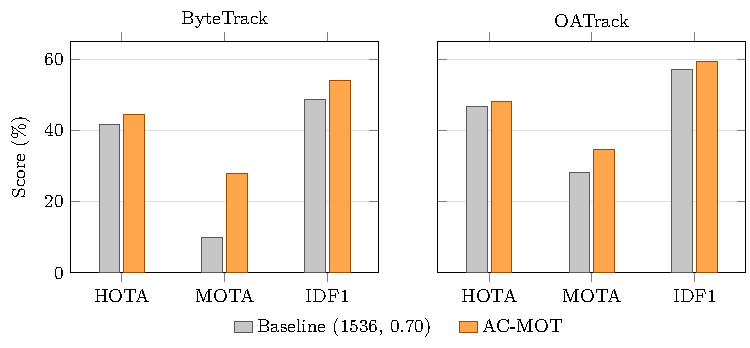
\includegraphics[width=0.85\textwidth]{figures/acmot_visdrone_bars.pdf}
\caption{HOTA, MOTA, and IDF1 on the seven VisDrone sequences for both tracker hosts (values in Table~\ref{tab:ac-visdrone}).}
\label{fig:ac-visdrone}
\end{figure}

\emph{Paired bootstrap.} In the VisDrone columns of Table~\ref{tab:ac-bootstrap}, the ByteTrack intervals of HOTA, MOTA, IDF1, precision, IDS, and FP lie entirely on the side of improvement, while FN and recall move in the opposite direction. With OATrack, HOTA, MOTA, IDF1, and precision rise and IDS and FP fall, all with intervals on one side of zero.

\begin{table}[tbp]
\centering
\caption{Paired sequence-level bootstrap of AC-MOT: AC-MOT minus baseline, 5000 resamples, seed 42, on VisDrone (7 sequences) and UAVDT (20 sequences). HOTA, MOTA, IDF1, precision, and recall in points; IDS, FP, and FN in counts. On UAVDT the bootstrap covers the count-based metrics only.}
\label{tab:ac-bootstrap}
\footnotesize\setlength{\tabcolsep}{4pt}
\begin{tabular}{llrlrl}
\toprule
 & & \multicolumn{2}{c}{VisDrone} & \multicolumn{2}{c}{UAVDT}\\
Host & Metric & Difference & 95\% interval & Difference & 95\% interval\\
\midrule
ByteTrack & HOTA & $+2.937$ & [$+2.356$, $+3.375$] & -- & \\
 & MOTA & $+17.995$ & [$+13.541$, $+23.282$] & $+17.601$ & [$+11.134$, $+26.767$]\\
 & IDF1 & $+5.360$ & [$+4.490$, $+6.178$] & $+3.367$ & [$+1.676$, $+5.013$]\\
 & IDS & $-325$ & [$-498$, $-164$] & $-115$ & [$-211.025$, $-26.975$]\\
 & FP & $-14382$ & [$-19176$, $-9620$] & $-67539$ & [$-104215.350$, $-37352.950$]\\
 & FN & $+1781$ & [$+288$, $+3594.075$] & $+7652$ & [$+1542.925$, $+18359.400$]\\
 & Precision & $+10.003$ & [$+8.712$, $+11.895$] & -- & \\
 & Recall & $-2.479$ & [$-4.507$, $-0.469$] & -- & \\
\midrule
OATrack & HOTA & $+1.325$ & [$+0.200$, $+2.264$] & -- & \\
 & MOTA & $+6.318$ & [$+4.741$, $+7.879$] & $+3.267$ & [$+0.607$, $+5.881$]\\
 & IDF1 & $+2.258$ & [$+0.548$, $+3.474$] & $+0.831$ & [$+0.125$, $+1.271$]\\
 & IDS & $-169$ & [$-292$, $-42$] & $-31$ & [$-101$, $+39$]\\
 & FP & $-3994$ & [$-6190$, $-2494.900$] & $-14268$ & [$-33958.075$, $-2188.950$]\\
 & FN & $-375$ & [$-1462.575$, $+670$] & $+3162$ & [$-211.100$, $+8959.050$]\\
 & Precision & $+3.981$ & [$+2.957$, $+5.511$] & -- & \\
 & Recall & $+0.522$ & [$-0.869$, $+2.111$] & -- & \\
\bottomrule
\end{tabular}
\end{table}

\subsection{Controller Behavior}\label{sec:ac-res-behavior}
The controller uses all three states with both hosts. With ByteTrack, LOW, MEDIUM, and HIGH cover 7.4\%, 30.1\%, and 62.5\% of the frames; with OATrack they cover 7.4\%, 33.3\%, and 59.3\%. For most of the video, the detector therefore runs with the HIGH action, the smallest input and a score threshold of 0.40. The two hosts diverge through their different tracked boxes. State changes are rare, between 0.10 and 0.54 per 100 frames depending on the sequence, so the detector input stays stable over long stretches of video.

\subsection{Frozen UAVDT Transfer}\label{sec:ac-res-uavdt}
The UAVDT transfer applies the frozen controller, with none of its values changed, to the 20 test sequences of a dataset that was not used to build it. Table~\ref{tab:ac-uavdt} and Fig.~\ref{fig:ac-uavdt} report the results.

\begin{table}[tbp]
\centering
\caption{Frozen UAVDT transfer of AC-MOT without retuning (20 sequences, 16,592 frames, one vehicle class). Baseline: fixed operating point (1536, 0.70).}
\label{tab:ac-uavdt}
\begin{tabular}{lrrrr}
\toprule
 & \multicolumn{2}{c}{ByteTrack} & \multicolumn{2}{c}{OATrack}\\
Metric & Baseline & AC-MOT & Baseline & AC-MOT\\
\midrule
HOTA & 45.923 & 47.004 & 47.728 & 47.640\\
MOTA & $-1.573$ & 16.028 & 19.607 & 22.873\\
IDF1 & 58.400 & 61.767 & 62.101 & 62.931\\
IDS & 601 & 486 & 517 & 486\\
FP & 279616 & 212077 & 197937 & 183669\\
FN & 66050 & 73702 & 75612 & 78774\\
Precision & 49.571 & 55.751 & 57.270 & 58.800\\
Recall & 80.625 & 78.381 & 77.820 & 76.893\\
\bottomrule
\end{tabular}
\end{table}

With ByteTrack, HOTA rises by 1.081 points, MOTA by 17.601, and IDF1 by 3.367; with OATrack, MOTA rises by 3.267 and IDF1 by 0.831, while HOTA is almost unchanged (47.728 and 47.640). With both hosts FP and IDS fall and precision rises, with slightly lower recall, the same pattern as with ByteTrack on VisDrone: the controller changes the detector output in the same way on a dataset that was not used to build it.

\begin{figure}[tbp]
\centering
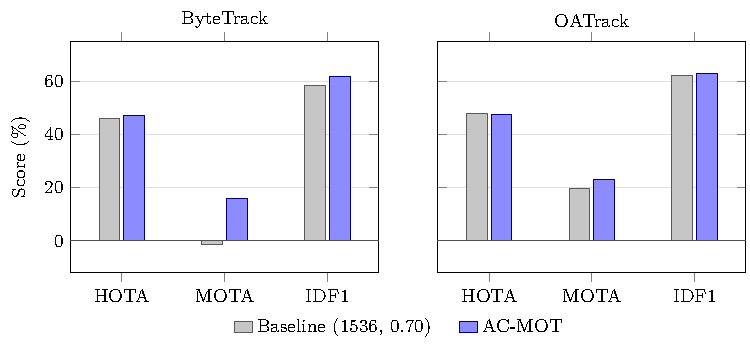
\includegraphics[width=0.85\textwidth]{figures/acmot_uavdt_bars.pdf}
\caption{HOTA, MOTA, and IDF1 of the frozen UAVDT transfer of AC-MOT for both tracker hosts (values in Table~\ref{tab:ac-uavdt}). The ByteTrack baseline MOTA is negative ($-1.573$); the solid line marks zero.}
\label{fig:ac-uavdt}
\end{figure}

In the UAVDT columns of Table~\ref{tab:ac-bootstrap}, the ByteTrack intervals of MOTA, IDF1, IDS, and FP lie on the side of improvement and FN moves the other way; with OATrack, MOTA and IDF1 rise and FP fall with intervals on one side of zero, while the IDS and FN intervals include zero.

\subsection{Runtime}\label{sec:ac-res-runtime}
AC-MOT needs no training and no access to detector or tracker internals; it changes three arguments of the detector call and analyzes a quarter-scale image every ten frames. On a Tesla T4 the controller takes 4.26 ms per frame with ByteTrack and 4.20 ms with OATrack, which is small next to detector inference and suitable for real-time use.

\section{Discussion}\label{sec:ac-discussion}
\emph{The operating point is part of the MOT system.} The same frozen detector and trackers give very different MOT results at different operating points: moving away from the fixed 1536/0.70 point raises MOTA by 17.995 points with ByteTrack and by 6.318 points with OATrack on VisDrone. On both datasets FP and IDS drop sharply and precision rises, while FN rise a little, so MOTA, which counts every FP, reacts most strongly. The detector operating point is therefore a first-order variable of aerial MOT and deserves the same attention as the association method. This answers RQ1 for the tested setting: the operating point can be adapted online from scene cues and past tracker output, without training, and the adaptation improves tracking over a fixed operating point.

\emph{A more selective detection stream.} Most of the time the controller selects the HIGH action, with the smallest input and a score threshold of 0.40 (Section~\ref{sec:ac-res-behavior}). The development studies explain why: a score threshold of 0.40 gave the tracker fewer but more reliable boxes and raised calibration HOTA on seven of eight sequences (Section~\ref{sec:ac-modern}), and the smaller input costs less detector time. The gain comes mainly from removing clutter and identity-confusing boxes.

\emph{Tracker dependence.} ByteTrack, which starts from a weaker baseline and uses low-score boxes in its second association step, gains more than OATrack, which already weights detections by quality and gains mainly in MOTA, IDF1, IDS, and FP. The preferred operating point thus depends on the tracker host, as the historical profiles of Section~\ref{sec:ac-dev} also showed. AC-MOT serves both hosts without changing them.

\emph{Transfer.} The frozen controller kept its effect on UAVDT, a dataset of vehicles recorded under other conditions, with none of its values changed (RQ3). The same pattern of fewer FP and IDS and higher precision appeared on both datasets.

\emph{Deployment.} AC-MOT needs no training and no access to detector or tracker internals, and it adds about 4.2 ms per frame on a Tesla T4. Its state changes are rare, so the detector input stays stable over long stretches of video.

\emph{Scope of the evaluation.} The frozen controller was evaluated with one detector, YOLO11m with VisDrone weights, two trackers, ByteTrack and OATrack, and two aerial datasets, with three operating points chosen from a grid of three input sizes, three NMS values, and three score thresholds. Its thresholds and actions are expressed for this detector; a different detector, tracker, or dataset is a direction for further evaluation (Section~\ref{sec:conc-future}). The controller also assumes that the scores of the detector keep the scale for which the tracker thresholds were set, the assumption that Chapter~\ref{ch:scl} removes.

\section{Summary}\label{sec:ac-summary}
This chapter presented AC-MOT, a training-free controller that adjusts the confidence threshold, the NMS IoU threshold, and the input resolution of the detector online to improve MOT in UAV video, using only the current frame and previous tracking results and without changing or retraining the detector or the tracker. A scene complexity index based on object density, a few other scene cues, and a three-state controller with recovery, hysteresis, and dwell rules let the settings follow the scene without frequent changes. The controller was developed through optimization experiments, and its final values were selected by cross-validation on separate calibration sequences and then kept fixed. On seven VisDrone2019-MOT sequences, AC-MOT improved HOTA by 2.937 points with ByteTrack and 1.325 points with OATrack, and MOTA by 17.995 and 6.318 points, respectively; paired bootstrap analysis supports these gains. On UAVDT it improved MOTA by 17.601 points with ByteTrack and 3.267 points with OATrack without retuning, at about 4.2 ms per frame. The results show that the detector operating point should be treated as part of the tracking system rather than as a fixed setting. AC-MOT, however, keeps the tracker thresholds as they are and relies on the detector's scores having the scale for which these thresholds were tuned. The next chapter addresses this relation between the detector's score scale and the tracker's thresholds.
